\section{Accelerating Detector Simulation}\label{sec:ml4sim}

\begin{figure}[htb!]
\centering
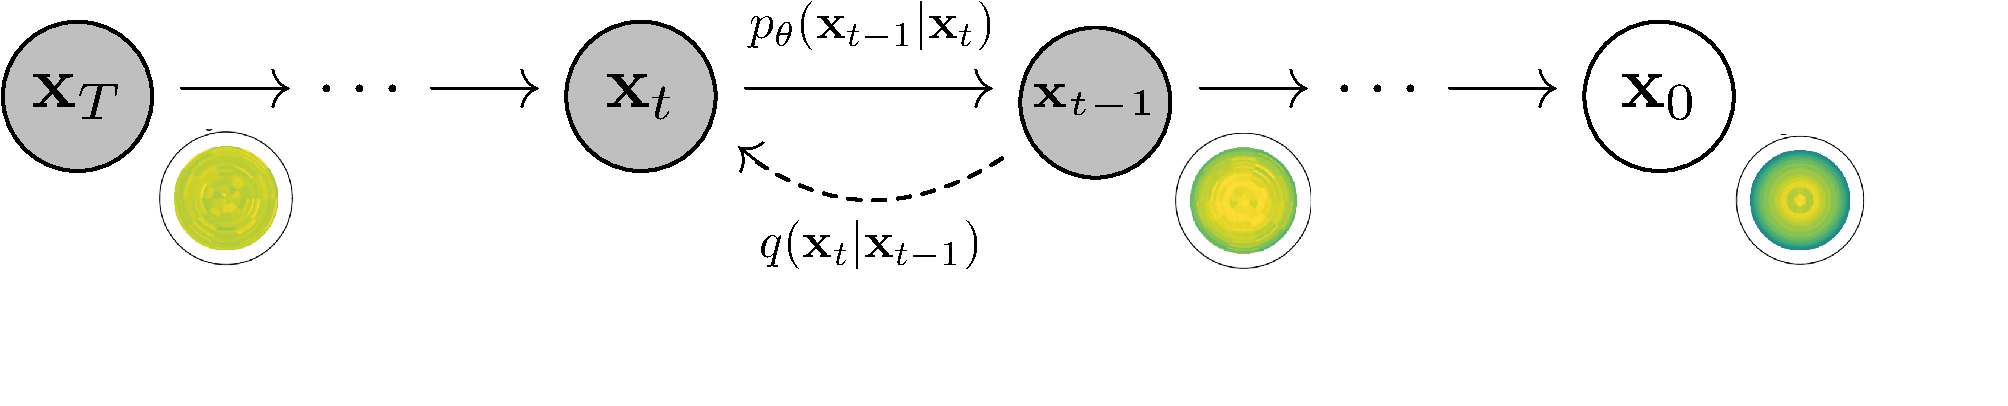
\includegraphics[width=0.95\myfigurewidth]{figures/pgm_diagram_xarrow_showers.pdf}
\caption{An illustration of the diffusion process, going from pure noise (left) to a realistic particle shower (right) in a transverse slice of a calorimeter. Adapted from Ref.~\cite{Ho:2020}.}
\label{fig:illus}
\end{figure}

\begin{figure}[htb!]
\centering
\twofigeqh{figures/ds1-pions_CE_1.pdf}{figures/FCC_ERatio_dataset2_oct11_layer_norm_Diffu.pdf}
\caption{Left: example comparison of the separation power (for the shower center of energy) between \diffu, other algorithms, and \GEANTfour in the community \challenge.
Right: improved \diffu performance on the total deposited energy.}
\label{fig:calodiffu}
\end{figure}